%!TEX TS-program = xelatex
%!TEX encoding = UTF-8 Unicode
% Awesome CV LaTeX Template
%
% This template has been downloaded from:
% https://github.com/posquit0/Awesome-CV
%
% Author:
% Claud D. Park <posquit0.bj@gmail.com>
% http://www.posquit0.com
%
% Template license:
% CC BY-SA 4.0 (https://creativecommons.org/licenses/by-sa/4.0/)
%


%%%%%%%%%%%%%%%%%%%%%%%%%%%%%%%%%%%%%%
%     Configuration
%%%%%%%%%%%%%%%%%%%%%%%%%%%%%%%%%%%%%%
%%% Themes: Awesome-CV
\documentclass[11pt, a4paper]{awesome-cv}

%%% Override a directory location for fonts(default: 'fonts/')
\fontdir[fonts/]

%%% Configure a directory location for sections
\newcommand*{\sectiondir}{resume/}

%%% Override color
% Awesome Colors: awesome-emerald, awesome-skyblue, awesome-red, awesome-pink, awesome-orange
%                 awesome-nephritis, awesome-concrete, awesome-darknight
%% Color for highlight
% Define your custom color if you don't like awesome colors
%\colorlet{awesome}{awesome-skyblue}
\definecolor{awesome}{HTML}{0e4f6f}
%% Colors for text
%\definecolor{darktext}{HTML}{414141}
%\definecolor{text}{HTML}{414141}
%\definecolor{graytext}{HTML}{414141}
%\definecolor{lighttext}{HTML}{414141}

%%% Override a separator for social informations in header(default: ' | ')
%\headersocialsep[\quad\textbar\quad]

\usepackage{import}
\usepackage{graphbox} 

%%%%%%%%%%%%%%%%%%%%%%%%%%%%%%%%%%%%%%
%     Personal Data
%%%%%%%%%%%%%%%%%%%%%%%%%%%%%%%%%%%%%%
%%% Essentials
\name{Sven}{Rademakers}
\address{Engelenkampstraat 55 6131JE, Sittard, Netherlands}
\mobile{(+46) 7 00 09 27 69} 
%%% Social
\email{sven.rademakers@gmail.com}
\linkedin{sxrademakers}
\github{svenrademakers}
\homepage{www.svenrademakers.nl}
%%% Optionals
\position{Senior Software Engineer}


%%%%%%%%%%%%%%%%%%%%%%%%%%%%%%%%%%%%%%
%     Content
%%%%%%%%%%%%%%%%%%%%%%%%%%%%%%%%%%%%%%
%%% Make a footer for CV with three arguments(<left>, <center>, <right>)
\makecvfooter
  {\today}
  {CV Sven Rademakers}
  {\thepage}

\begin{document}
%%% Make a header for CV with personal data
\makecvheader
\cvsection{About Me}
\begin{tabular*}{\textwidth}{ L{4cm} R{13cm}}
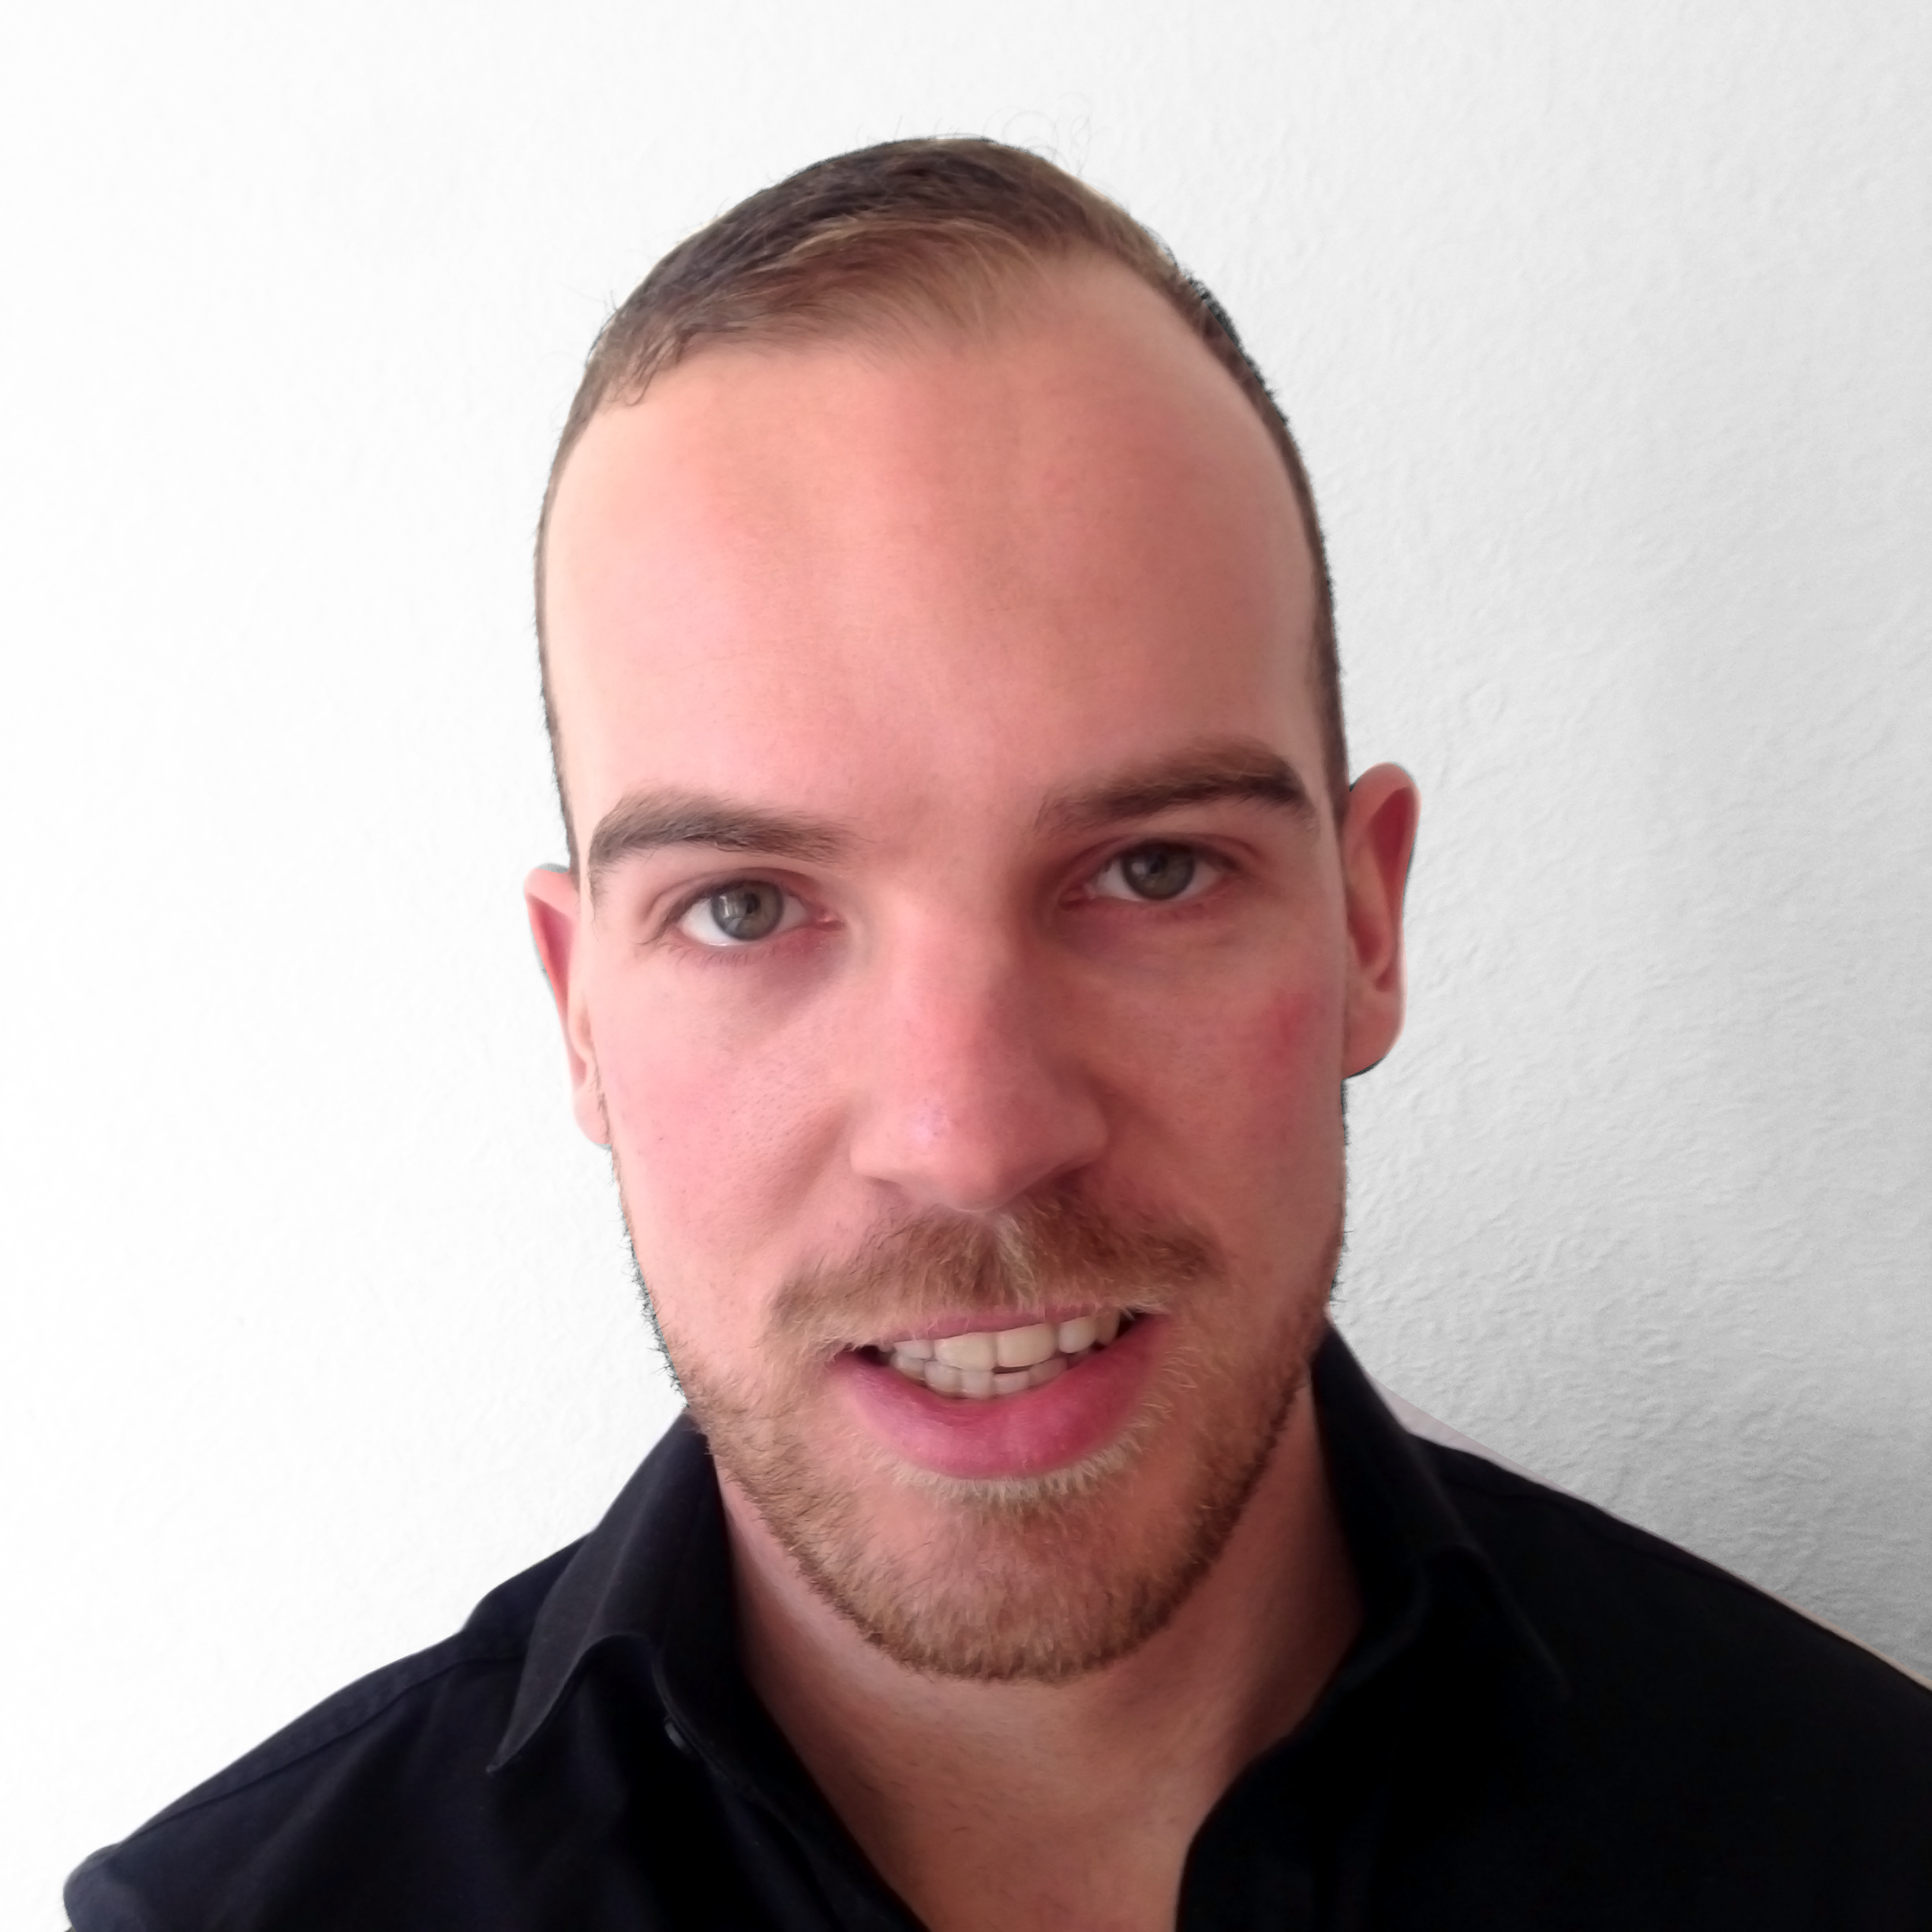
\includegraphics[width=4cm, align=0cm]{Sven.png} &
	\begin{cventries}
    	\begin{cvitems}
    	\descriptionstyle{
        \textbf{Looking for a new assignment in the London area!}
        \item{Born: 19-05-1991.}
        \item{Nationality: Dutch.}
        \item{Languages: Dutch (native), English (Speaking \& Reading proficient).}
        \item{I'm very curious by nature, always seeking to learn new things and I never back down from a challenge. Moreover, my flexibility has proven to be a key aspect in my ability to work in a team while still maintaining control over my personal schedule.}
        \item{A successful project for me is when we took risks, pushed the envelope on technology, while staying realistic and therefore made the right decisions.}
        \item{My goal in my career is to grow as an engineer, to become a leading expert on engineering practises and technology.}
        \item{Music is next to software engineering one of my biggest hobbies. Everything from recording, gear to guitars.}
		}
    \end{cvitems}
        \end{cventries}
  \end{tabular*}
  
\import{\sectiondir}{experience.tex}

\end{document}
